\refstepcounter{section}
\section*{Lecture 05: More on Van der Waal's Equation}
\addcontentsline{toc}{section}{Lecture 05: More on Van der Waal}
In the previous section, we saw a mathematical theory of condensation based on the zeroes of the grand partition function. Let us now move back to the Van der Waal's equation and try to analyse the critical point. 
\begin{figure}[H]\label{fig:isotherms}
    \centering
    

\tikzset{every picture/.style={line width=0.75pt}} %set default line width to 0.75pt        

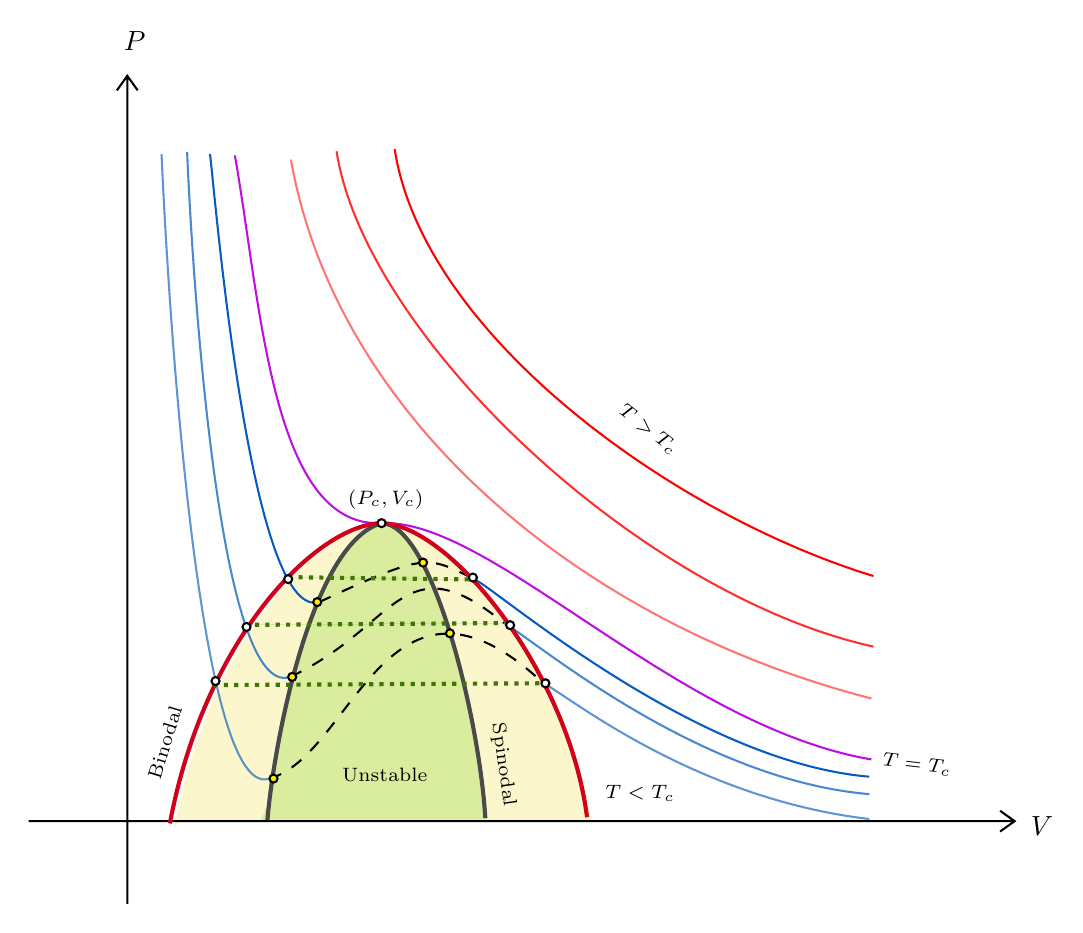
\begin{tikzpicture}[x=0.75pt,y=0.75pt,yscale=-1,xscale=1]
%uncomment if require: \path (0,583); %set diagram left start at 0, and has height of 583

%Shape: Path Data [id:dp14847922389040458] 
\draw  [draw opacity=0][fill={rgb, 255:red, 241; green, 221; blue, 49 }  ,fill opacity=0.25 ][line width=1.5]  (191.63,423.74) .. controls (191.86,422.46) and (192.11,421.18) .. (192.36,419.91) -- (192.36,419.91) .. controls (210.14,330.56) and (263.06,277.09) .. (293.63,276.4) -- (293.63,276.4) -- (293.63,276.4) -- (293.63,276.4) .. controls (326.21,277.09) and (382.19,347.58) .. (392.26,417.98) -- (393.6,419.91) -- (392.52,419.91) .. controls (392.56,420.15) and (392.59,420.39) .. (392.62,420.64) .. controls (392.62,420.65) and (392.62,420.67) .. (392.63,420.69) -- (392.09,419.91) -- (194.28,419.91) -- (192.39,422.64) -- (192.39,422.64) -- (191.63,423.74) -- cycle ;
%Shape: Path Data [id:dp9555956516260592] 
\draw  [draw opacity=0][fill={rgb, 255:red, 126; green, 211; blue, 33 }  ,fill opacity=0.14 ][line width=1.5]  (290.68,276.4) .. controls (313.75,276.42) and (335.89,362.01) .. (340.24,412.53) -- (342.68,419.23) -- (235.79,419.23) -- (235.68,419.5) .. controls (235.69,419.41) and (235.7,419.32) .. (235.71,419.23) -- (233.68,419.23) -- (236.37,412.49) .. controls (240.87,372.25) and (258.7,285.32) .. (290.68,276.4) -- (290.68,276.4) -- (290.68,276.4) -- (290.68,276.4) -- (290.68,276.4) -- cycle ;
%Shape: Path Data [id:dp8936092149045763] 
\draw  [draw opacity=0][fill={rgb, 255:red, 126; green, 211; blue, 33 }  ,fill opacity=0.14 ] (235.68,419.5) .. controls (235.69,419.41) and (235.7,419.32) .. (235.71,419.23) -- (233.68,419.23) -- (236.37,412.49) .. controls (240.87,372.25) and (258.7,285.32) .. (290.68,276.4) -- (290.68,276.4) -- (290.68,276.4) -- (290.68,276.4) -- (290.68,276.4) .. controls (313.75,276.42) and (335.89,362.01) .. (340.24,412.53) -- (342.68,419.23) -- (235.79,419.23) -- (235.68,419.5) -- cycle ;

%Shape: Axis 2D [id:dp5915928413529832] 
\draw  (121.68,419.98) -- (596.68,419.98)(169.18,60.88) -- (169.18,459.88) (589.68,414.98) -- (596.68,419.98) -- (589.68,424.98) (164.18,67.88) -- (169.18,60.88) -- (174.18,67.88)  ;
%Curve Lines [id:da7762081291051] 
\draw [color={rgb, 255:red, 255; green, 0; blue, 0 }  ,draw opacity=1 ]   (298,96.23) .. controls (311.68,184.88) and (430.68,271.88) .. (528.68,301.88) ;
%Curve Lines [id:da03831394409611277] 
\draw [color={rgb, 255:red, 255; green, 0; blue, 0 }  ,draw opacity=0.81 ]   (270,97.23) .. controls (283.68,185.88) and (415.68,310.88) .. (528.68,335.88) ;
%Curve Lines [id:da06969152148211877] 
\draw [color={rgb, 255:red, 255; green, 0; blue, 0 }  ,draw opacity=0.54 ]   (248,101.23) .. controls (269.68,223.88) and (384.68,323.88) .. (527.68,360.88) ;
%Curve Lines [id:da7386168932359989] 
\draw [color={rgb, 255:red, 189; green, 16; blue, 224 }  ,draw opacity=1 ]   (221,99.23) .. controls (233.68,170.83) and (238.68,278.85) .. (291.68,276.4) .. controls (344.68,273.95) and (432.68,373.95) .. (527.68,390.25) ;
%Curve Lines [id:da4619239839468895] 
\draw [color={rgb, 255:red, 7; green, 92; blue, 191 }  ,draw opacity=1 ]   (209,98.53) .. controls (210.68,108.63) and (227.68,324.42) .. (261.68,314.42) ;
%Curve Lines [id:da4084854232070537] 
\draw [color={rgb, 255:red, 7; green, 92; blue, 191 }  ,draw opacity=1 ]   (336.68,303.55) .. controls (348.68,309.55) and (442.68,391.55) .. (526.68,398.55) ;
%Curve Lines [id:da3801879993326518] 
\draw [color={rgb, 255:red, 7; green, 92; blue, 191 }  ,draw opacity=0.73 ]   (350.68,324.55) .. controls (362.68,330.55) and (442.68,399.95) .. (526.68,406.95) ;
%Curve Lines [id:da21958016559613858] 
\draw [color={rgb, 255:red, 7; green, 92; blue, 191 }  ,draw opacity=0.65 ]   (369.68,353.55) .. controls (381.68,359.55) and (441.68,408.95) .. (526.68,418.95) ;
%Curve Lines [id:da06519860019459167] 
\draw [color={rgb, 255:red, 7; green, 92; blue, 191 }  ,draw opacity=0.73 ]   (198,97.53) .. controls (198.68,114.47) and (209.68,363.47) .. (247.68,350.47) ;
%Curve Lines [id:da9879500666094625] 
\draw [color={rgb, 255:red, 7; green, 92; blue, 191 }  ,draw opacity=0.65 ]   (185.68,98.58) .. controls (186.37,115.52) and (199.68,412.47) .. (237.68,399.47) ;
%Curve Lines [id:da2839008192624404] 
\draw  [dash pattern={on 4.5pt off 4.5pt}]  (261.68,314.42) .. controls (313.68,290.15) and (313.68,292.15) .. (336.68,303.55) ;
%Curve Lines [id:da9260172449037632] 
\draw  [dash pattern={on 4.5pt off 4.5pt}]  (247.68,350.47) .. controls (299.68,326.2) and (301.68,284.5) .. (350.68,324.55) ;
%Curve Lines [id:da16684951274261806] 
\draw  [dash pattern={on 4.5pt off 4.5pt}]  (237.68,399.47) .. controls (277.68,388.5) and (294.68,283.5) .. (369.68,353.55) ;
%Shape: Boxed Bezier Curve [id:dp902739197661444] 
\draw [color={rgb, 255:red, 74; green, 74; blue, 74 }  ,draw opacity=1 ][line width=1.5]    (236.68,419.5) .. controls (239.68,383.5) and (257.68,285.88) .. (291.68,276.4) ;
%Curve Lines [id:da8362785705456496] 
\draw [color={rgb, 255:red, 74; green, 74; blue, 74 }  ,draw opacity=1 ][line width=1.5]    (341.68,418.5) .. controls (338.68,369.1) and (315.68,276.42) .. (291.68,276.4) ;
%Shape: Boxed Bezier Curve [id:dp723139145956698] 
\draw [color={rgb, 255:red, 208; green, 2; blue, 27 }  ,draw opacity=1 ][line width=1.5]    (189.68,421.08) .. controls (206.68,331.08) and (260.68,277.08) .. (291.68,276.4) ;
%Curve Lines [id:da03824974658577196] 
\draw [color={rgb, 255:red, 208; green, 2; blue, 27 }  ,draw opacity=1 ][line width=1.5]    (390.68,418.08) .. controls (381.68,348.08) and (324.68,277.08) .. (291.68,276.4) ;
%Straight Lines [id:da06381764278461444] 
\draw [color={rgb, 255:red, 65; green, 117; blue, 5 }  ,draw opacity=1 ][fill={rgb, 255:red, 65; green, 117; blue, 5 }  ,fill opacity=1 ][line width=1.5]  [dash pattern={on 1.5pt off 2.25pt}]  (246.68,302.42) -- (336.68,303.55) ;
%Straight Lines [id:da17288457548559477] 
\draw [color={rgb, 255:red, 65; green, 117; blue, 5 }  ,draw opacity=1 ][fill={rgb, 255:red, 65; green, 117; blue, 5 }  ,fill opacity=1 ][line width=1.5]  [dash pattern={on 1.5pt off 2.25pt}]  (225.68,325.42) -- (350.68,324.55) ;
%Straight Lines [id:da049765591139104726] 
\draw [color={rgb, 255:red, 65; green, 117; blue, 5 }  ,draw opacity=1 ][line width=1.5]  [dash pattern={on 1.5pt off 2.25pt}]  (210.68,354.42) -- (369.68,353.55) ;
%Shape: Circle [id:dp16781382062311356] 
\draw  [fill={rgb, 255:red, 255; green, 255; blue, 255 }  ,fill opacity=1 ] (209.74,352.48) .. controls (209.74,351.4) and (210.61,350.53) .. (211.68,350.53) .. controls (212.76,350.53) and (213.63,351.4) .. (213.63,352.48) .. controls (213.63,353.55) and (212.76,354.42) .. (211.68,354.42) .. controls (210.61,354.42) and (209.74,353.55) .. (209.74,352.48) -- cycle ;
%Shape: Circle [id:dp6534370820124757] 
\draw  [fill={rgb, 255:red, 255; green, 255; blue, 255 }  ,fill opacity=1 ] (224.68,326.42) .. controls (224.68,325.34) and (225.55,324.48) .. (226.63,324.48) .. controls (227.7,324.48) and (228.57,325.34) .. (228.57,326.42) .. controls (228.57,327.49) and (227.7,328.36) .. (226.63,328.36) .. controls (225.55,328.36) and (224.68,327.49) .. (224.68,326.42) -- cycle ;
%Shape: Circle [id:dp6434045943315729] 
\draw  [fill={rgb, 255:red, 255; green, 255; blue, 255 }  ,fill opacity=1 ] (244.74,303.36) .. controls (244.74,302.29) and (245.61,301.42) .. (246.68,301.42) .. controls (247.76,301.42) and (248.63,302.29) .. (248.63,303.36) .. controls (248.63,304.43) and (247.76,305.3) .. (246.68,305.3) .. controls (245.61,305.3) and (244.74,304.43) .. (244.74,303.36) -- cycle ;
%Shape: Circle [id:dp09505076508185872] 
\draw  [fill={rgb, 255:red, 255; green, 255; blue, 255 }  ,fill opacity=1 ] (289.74,276.4) .. controls (289.74,275.33) and (290.61,274.46) .. (291.68,274.46) .. controls (292.76,274.46) and (293.63,275.33) .. (293.63,276.4) .. controls (293.63,277.47) and (292.76,278.34) .. (291.68,278.34) .. controls (290.61,278.34) and (289.74,277.47) .. (289.74,276.4) -- cycle ;
%Shape: Circle [id:dp7876455677275235] 
\draw  [fill={rgb, 255:red, 255; green, 255; blue, 255 }  ,fill opacity=1 ] (333.74,302.61) .. controls (333.74,301.54) and (334.61,300.67) .. (335.68,300.67) .. controls (336.76,300.67) and (337.63,301.54) .. (337.63,302.61) .. controls (337.63,303.68) and (336.76,304.55) .. (335.68,304.55) .. controls (334.61,304.55) and (333.74,303.68) .. (333.74,302.61) -- cycle ;
%Shape: Circle [id:dp453131059600555] 
\draw  [fill={rgb, 255:red, 255; green, 255; blue, 255 }  ,fill opacity=1 ] (351.68,325.55) .. controls (351.68,324.48) and (352.55,323.61) .. (353.63,323.61) .. controls (354.7,323.61) and (355.57,324.48) .. (355.57,325.55) .. controls (355.57,326.62) and (354.7,327.49) .. (353.63,327.49) .. controls (352.55,327.49) and (351.68,326.62) .. (351.68,325.55) -- cycle ;
%Shape: Circle [id:dp8216329432850344] 
\draw  [fill={rgb, 255:red, 255; green, 255; blue, 255 }  ,fill opacity=1 ] (368.68,353.55) .. controls (368.68,352.48) and (369.55,351.61) .. (370.63,351.61) .. controls (371.7,351.61) and (372.57,352.48) .. (372.57,353.55) .. controls (372.57,354.62) and (371.7,355.49) .. (370.63,355.49) .. controls (369.55,355.49) and (368.68,354.62) .. (368.68,353.55) -- cycle ;
%Shape: Circle [id:dp545909479963963] 
\draw  [fill={rgb, 255:red, 255; green, 235; blue, 0 }  ,fill opacity=1 ] (309.74,295.4) .. controls (309.74,294.33) and (310.61,293.46) .. (311.68,293.46) .. controls (312.76,293.46) and (313.63,294.33) .. (313.63,295.4) .. controls (313.63,296.47) and (312.76,297.34) .. (311.68,297.34) .. controls (310.61,297.34) and (309.74,296.47) .. (309.74,295.4) -- cycle ;
%Shape: Circle [id:dp178844485717639] 
\draw  [fill={rgb, 255:red, 255; green, 235; blue, 0 }  ,fill opacity=1 ] (258.74,314.42) .. controls (258.74,313.34) and (259.61,312.48) .. (260.68,312.48) .. controls (261.76,312.48) and (262.63,313.34) .. (262.63,314.42) .. controls (262.63,315.49) and (261.76,316.36) .. (260.68,316.36) .. controls (259.61,316.36) and (258.74,315.49) .. (258.74,314.42) -- cycle ;
%Shape: Circle [id:dp7456472761560751] 
\draw  [fill={rgb, 255:red, 255; green, 235; blue, 0 }  ,fill opacity=1 ] (246.68,350.47) .. controls (246.68,349.39) and (247.55,348.52) .. (248.63,348.52) .. controls (249.7,348.52) and (250.57,349.39) .. (250.57,350.47) .. controls (250.57,351.54) and (249.7,352.41) .. (248.63,352.41) .. controls (247.55,352.41) and (246.68,351.54) .. (246.68,350.47) -- cycle ;
%Shape: Circle [id:dp3863443930477858] 
\draw  [fill={rgb, 255:red, 255; green, 235; blue, 0 }  ,fill opacity=1 ] (237.68,399.47) .. controls (237.68,398.39) and (238.55,397.52) .. (239.63,397.52) .. controls (240.7,397.52) and (241.57,398.39) .. (241.57,399.47) .. controls (241.57,400.54) and (240.7,401.41) .. (239.63,401.41) .. controls (238.55,401.41) and (237.68,400.54) .. (237.68,399.47) -- cycle ;
%Shape: Circle [id:dp6122178853359954] 
\draw  [fill={rgb, 255:red, 255; green, 235; blue, 0 }  ,fill opacity=1 ] (322.68,329.47) .. controls (322.68,328.39) and (323.55,327.52) .. (324.63,327.52) .. controls (325.7,327.52) and (326.57,328.39) .. (326.57,329.47) .. controls (326.57,330.54) and (325.7,331.41) .. (324.63,331.41) .. controls (323.55,331.41) and (322.68,330.54) .. (322.68,329.47) -- cycle ;

% Text Node
\draw (166,38.18) node [anchor=north west][inner sep=0.75pt]    {$P$};
% Text Node
\draw (603,416.18) node [anchor=north west][inner sep=0.75pt]    {$V$};
% Text Node
\draw (409.15,215.92) node [anchor=north west][inner sep=0.75pt]  [font=\scriptsize,rotate=-38]  {$T >T_{c}$};
% Text Node
\draw (398,401.18) node [anchor=north west][inner sep=0.75pt]  [font=\scriptsize]  {$T< T_{c}$};
% Text Node
\draw (532.22,385.3) node [anchor=north west][inner sep=0.75pt]  [font=\scriptsize,rotate=-6.62]  {$T=T_{c}$};
% Text Node
\draw (274,258.75) node [anchor=north west][inner sep=0.75pt]  [font=\scriptsize]  {$( P_{c} ,V_{c})$};
% Text Node
\draw (271.16,392.72) node [anchor=north west][inner sep=0.75pt]  [font=\scriptsize] [align=left] {Unstable};
% Text Node
\draw (176.93,399.26) node [anchor=north west][inner sep=0.75pt]  [font=\scriptsize,rotate=-287.24] [align=left] {Binodal};
% Text Node
\draw (352.76,370.54) node [anchor=north west][inner sep=0.75pt]  [font=\scriptsize,rotate=-81.95] [align=left] {Spinodal};


\end{tikzpicture}

    \caption{\textbf{Van der Waal's isotherm}. The figure shows Van der Waal's isotherms for $T<T_c$ ($T>T_c$) with blue (red) lines. The curve for $T=T_c$ is shown with purple line. Maxwell's construction is shown with green dotted line. The red line denotes the \textit{binodal line} and the gray line denotes the \textit{spinodal} line. The yellow region denote the metastable state while the green region denote the unstable states.}
\end{figure}
\noindent
In Fig.\ref{fig:isotherms}, we see the Van der Waal's isotherms at different temperature regime. There exists a temperature $T_c$ such that at a particular point $(V_c, P_c)$, the isotherm has zero slope and zero curvature. Thus the critical point is characterised by 
$$\pdv{P}{V}=0\qquad \pdv[2]{P}{V}=0$$
Defining $v=\frac{V}{N}$, from Van der Waal's equation we can write,
\begin{align}
    P = \frac{\kb T}{v-b} - \frac{a}{v^2} \implies \pdv{P}{V} = -\frac{\kb T}{(v-b)^2} +\frac{2a}{v^3}\implies \pdv[2]{P}{V} = \frac{2\kb T}{(v-b)^3}-\frac{6a}{v^4}
\end{align}
Equating the derivative to zero, we get $2a(v_c-b)^2=\kb T v_c^3$ and equating the second derivative to zero, we get $3a(v_c-b)^3 = \kb T v_c^4$. Dividing both these equations, we get 
$$\frac{3}{2}(v_c-b) =v_c \implies 3(v_c-b)=2v_c \implies {v_c=3b}$$
Substituting this in any one of the above equation we get $\kb T_c = \frac{8a}{27b}$ and substituting $v_c$ and $T_c$ in Van der Waal's equation, we get $P_c = \frac{a}{27b^2}$. Thus our critical parameters are,
$$\boxed{P_c = \frac{a}{27b^2}\qquad {v_c=3b}\qquad \kb T_c = \frac{8a}{27b}}$$
\subsection{Approaching Universality}
The Van der Waal's equation depends on the microscopic details of the system, $a$ and $b$. These vary for different gases and hence, the equation cannot describe universal properties. However, let us define the \textit{reduced parameters},
$$\Pi = \frac{P}{P_c}\qquad \nu = \frac{v}{v_c}\qquad \tau = \frac{T}{T_c}$$
We now put these in the equation of state, which gives us 
\begin{align}\label{eqn:reducedvdw}
   \begin{split}
     \qty(\Pi P_c + \frac{a}{\nu^2 v_c^2})\qty(\nu v_c - b) = \kb \tau T_c &\implies \qty(\frac{\Pi a}{27b^2} + \frac{a}{9\nu^2 b^2})\qty(3b\nu  - b) =  \frac{8a \tau}{27b}\\
    &\implies \frac{3ab}{27b^2}\qty(\Pi+\frac{3}{\nu^2})\qty(\nu - \frac{1}{3})=\frac{8a \tau }{27b}\\
    &\implies \boxed{\qty(\Pi+\frac{3}{\nu^2})\qty(\nu - \frac{1}{3})=\frac{8 \tau }{3}}
   \end{split}
\end{align}
The above dimensionless Van der Waal's equation in terms of the reduced parameters, is independent of $a$ and $b$ and is thus \textit{universal}, in the sense that, different gases are expected to follow the same equation. The generalisation is known as the \textit{principle of corresponding states}, which says that all fluids when compared with respect to reduced parameters, have the same \textit{compressibility factor}. The compressibility factor is defined as $Z = \frac{Pv}{\kb T}$, with the critical value predicted by Van der Waal to be,
$$\qquad Z_c = \frac{P_cv_c}{\kb T_c} = \frac{3ab }{27b^2\times \frac{8a}{27b}} = \frac{3}{8} = 0.375$$
Experimentally, the critical value of the compressibility factor is found to be in the range $0.28-0.33$, thus, Van der Waal's equation does not provide an accurate quantitative estimate. 
\begin{figure}[H]
    \centering
    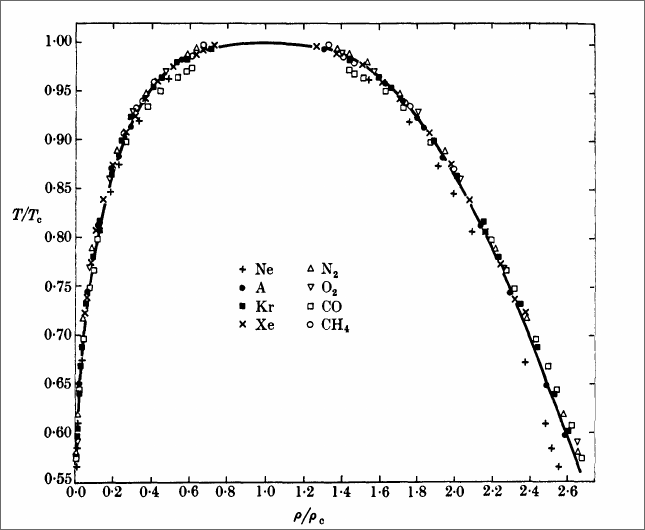
\includegraphics[scale=0.4]{pics/2026-01-14-132503_hyprshot.png}
    \caption{The Guggenheim plot for different gases with reduced parameter, showing that the trend follows a universal function (Source: Guggenheim (1945) \cite{Guggenheim}).}
\end{figure}
\subsection{Critical Opalescence}
Critical opalescence refers to an enhanced scattering of light by a substance in this critical region. Such enhanced scattering renders the substance milky white in reflected light. \\[0.2cm]
As we know, at the critical point, $\kappa\tund{T} = -\frac{1}{V}\qty(\pdv{V}{P})_T \to \infty$ since the slope of the isotherm is zero at the critical point. As $\kappa\tund{T}\propto \sigma\tund{N}$ where $\sigma\tund{N}$ is the number fluctuations in the system, there is a huge number fluctuation, due to which the scattering of light is intensified.
\subsection{Critical Point Behaviour}
We will now discuss the behaviour of gases in the vicinity of the critical point to analyse universality. For $T>T_c$, there is always a unique volume corresponding to each pressure and hence, we can apply \textit{Taylor expansion} around $v_c$ to write the pressure as,
\begin{align*}
    P(T,v) = P(T,v_c) + \pdv{P}{v}\Bigg|_{T} (v-v_c)+\frac{1}{2}\pdv[2]{P}{v}\Bigg|_{T} (v-v_c)^2+\frac{1}{6}\pdv[3]{P}{v}\Bigg|_{T} (v-v_c)^3+\SO\qty[\qty(\frac{v-v_c}{v_c})^4]
\end{align*}
Each of the coefficients are functions of temperature and hence, can be Taylor expanded about $T_c$. 
\begin{align*}
    P(T,v_c) &= \underbrace{P(T_c,v_c)}_{P_c}+\alpha(T-T_c)+\SO\qty[\qty(\frac{T-T_c}{T_c})^2]\\
    \pdv{P}{v}\Bigg|_{T, v_c}&=\cancelto{0}{\pdv{P}{v}}\Bigg|_{T_c, v_c} -a(T-T_c)+\SO\qty[\qty(\frac{T-T_c}{v_c})^2]\\
     \pdv[2]{P}{v}\Bigg|_{T, v_c}&=\cancelto{0}{\pdv[2]{P}{v}}\Bigg|_{T_c, v_c} +b(T-T_c)+\SO\qty[\qty(\frac{T-T_c}{T_c})^2]\\
     \pdv[3]{P}{v}\Bigg|_{T, v_c}&=-c +\SO\qty[\qty(\frac{T-T_c}{T_c})^2]
\end{align*}
At the critical point the slope and the curvature vanishes and hence the first terms in the second and third equation is zero. Using the stability condition in Eq. \eqref{eqn:stability}, $a>0$ for $T>T_c$ and $c>0$. $b$ can have any arbitrary sign\footnote{These $a,b$ are not the ones appearing in the Van der Waal's equation.}. Let us put these expression in the original Taylor expansion.
\begin{align}
    P(T,v) =P_c+ \alpha(T-T_c) -a(T-T_c) (v-v_c)+\frac{b}{2}(T-T_c) (v-v_c)^2-\frac{c}{6}(v-v_c)^3+\text{higher orders}\ldots
\end{align}
From this, we can predict the following things about different quantities:
\begin{itemize}
\item Let us consider only upto linear order in $(T-T-c)$ and $(v-v_c)$, hence we neglect the fourth, fifth and higher order terms. This gives us an approximate analytic solution for the pressure,
\begin{align*}
    \boxed{P(T,v) =P_c+ \alpha(T-T_c) -a(T-T_c) (v-v_c)}
\end{align*}
 We obtain $\pdv{P}{v} = -a(T-T_c)$ and hence the isothermal compressibility at $v_c$ scales as, $$\lim\limits_{T\to T_c^+}\kappa(T,v_c) = -\frac{1}{v_c}\pdv{v}{P} \sim \frac{1}{T-T_c}$$
 Experimental results identify the exponent as $\gamma\approx 1.3$ where $\kappa(T,v_c)\sim (T-T_c)^{-\gamma}$.
 \item At $T=T_c$, the isotherm behaves as $$P=P_c - \frac{c}{6}(v-v_c)^3 \implies (P-P_c)\sim (v-v_c)^3$$
 Experimental results identify the exponent as $\delta\approx 5.0$ where $(P-P_c)\sim (v-v_c)^{\delta}$.
\end{itemize}
The above analysis cannot be applied for $T<T_c$ since then for each pressure, we have two volumes and Taylor expansion cannot be effectively applied. Let us do the analysis in an alternate way using Eq. \eqref{eqn:reducedvdw}. Consider the two volumes $v\tund{liq}$ and $v\tund{gas}$ for which the pressure is same at say some temperature $T$. Then, from the equation we can write,
\begin{align*}
    \Pi = \frac{8\tau/3}{\nu_g-1/3} -\frac{3}{\nu_g^2} = \frac{8\tau/3}{\nu_l-1/3} -\frac{3}{\nu_l^2} 
\end{align*}
From this we obtain,
$$8\tau\qty[\frac{1}{\nu_g-1} -\frac{1}{\nu_l-1}] = 3\qty[\frac{1}{\nu_l^2}-\frac{1}{\nu_g^2}] =3\qty[\frac{\nu_g^2-\nu_l^2}{\nu_l^2\nu_g^2}] \implies \boxed{\tau = \frac{(3\nu_l-1)(3\nu_g-1)(\nu_l+\nu_g)}{8\nu_g^2\nu_l^2}}$$
Note that the equation is symmetric in $\nu_g$ and $\nu_l$ and $\nu_g=\nu_l=1$ at the critical point, which implies that we can write $$\nu_g = 1+\frac{\varepsilon}{2}\qquad \nu_l = 1-\frac{\varepsilon}{2}$$
where $\varepsilon \equiv \nu_g-\nu_l$. We substitute this in the expression for $\tau$, leading us to 
\begin{align*}
    \tau = \frac{2\qty(2-\frac{3\varepsilon}{2})\qty(2+\frac{3\varepsilon}{2})}{8\qty[\qty(1+\frac{\varepsilon}{2})\qty(1-\frac{\varepsilon}{2})]^2} =\frac{\qty(4-\frac{9\varepsilon^2}{4})}{4\qty(1-\frac{\varepsilon^2}{4})^2} = \qty( 1-\frac{9\varepsilon^2}{16})\qty(1-\frac{\varepsilon^2}{4})^{-2} \approx 
    \qty( 1-\frac{9\varepsilon^2}{16})\qty(1+\frac{\varepsilon^2}{2}) = 1-\frac{\varepsilon^2}{16}+\SO(\varepsilon^4)
\end{align*}
Then substituting for the real variables, we have $$(v\tund{gas}-v\tund{liq}) \sim (T_c-T)^{1/2}$$
Experimental results predict an exponent $\beta\approx 0.3$ where $(v\tund{gas}-v\tund{liq}) \sim (T_c-T)^\beta$.\\[0.2cm]
Van der Waal's equation thus does not provide a perfect quantitative description of condensation, however, qualitative descriptions are more or less accurate. The exponents $\beta,\gamma,\delta\ldots$ are called \textit{critical exponents} and many people dedicate their lives in finding the numerical value of these exponents.